\chapter{Introduction}
\label{chapter:introduction}
\com{Este modelo foi preparado utilizando como base uma disserta\c{c}\~{a}o. Alguns textos do documento original foram mantidos a fim de mostrar como se utiliza alguns comandos em latex. Para fazer um lembrete ou coment\'{a}rio no texto foi definido o comando ``$\backslash$com'', o texto ir\'{a} aparecer em vermelho, como neste cabe\c{c}alho.

Os comandos devem ser visualizados num editor de latex, n\~{a}o no pdf gerado (obviamente). Para quem est\'{a} come\c{c}ando a trabalhar com latex eu sugiro utilizar o TexMaker.

\textbf{As diferen\c{c}as entre este modelo e o modelo da BU est\~{a}o expostas como coment\'{a}rio no cabe\c{c}alho do  c\'{o}digo .tex}.

\'{E} poss\'{i}vel inserir anima\c{c}\~{o}es em .pdf, o ap\^{e}ndice A exp\~{o}e como isso pode ser feito. Entretanto, deve-se utilizar o Adobe Reader para visualizar o pdf.}

A good way to start a chapter is to introduce the topics that the chapter exposes (in order of appearance). Remember to put a review section at the end of the chapter with one or two paragraphs that briefly review what was exposed and the most important points. Also, it should be shown how this knowledge will be used in the next chapters (always link one chapter to the other). For more information and tips on technical writing see \citeonline{schroeter2013}.

\section{Citation tests section}
\label{sec:citation_test}
This is a dummy section that shows how citation is done in this model. Here we have a single author work \citeonline{yan1999creative} and here the same work \cite{yan1999creative}. This is how specific pages citations will appear: ``A design process is a logical sequence of events to ensure the success of designing devices, products, systems, or processes''\cite[p.~14]{yan1999creative}.

Going a little further, we have a two authors work \citeonline{hartenberg1964kinematic} and again here \cite{hartenberg1964kinematic}. 

This is a three authors text \citeonline{srikrishnan2011robotics} and again \cite{srikrishnan2011robotics}. This is how two or more works are cited \cite{brown2007, solent2013}. This is a five authors text \citeonline{zhao2009stitched} and again \cite{zhao2009stitched}. This is a six authors text \citeonline{saadi2006tratamento} and again  \cite{saadi2006tratamento}.

If you go to the bibliography you'll notice that all the authors appear in the references (even for works with more than 3 authors). This is one difference between the current template and the BU/ABNT template.

Some random paragraph citing standards: although ``sewing machine'' is a common term used daily, in the technical field of stitching is more usual to refer to such machines as ``stitching machines''. The verb ``to sew'' is also replaced with ``to stitch''. This terminology is defined by standard \citeonline{iso4915} and is also used in standard \citeonline{astmd6193}. The Brazilian standard for types of stitches, \citeonline{nbr13483}, is based on \citeonline{iso4915}, however, as \citeonline{nbr13483} is written in Portuguese, this work will use the terminology defined by \citeonline{iso4915} since \citeonline{iso4915} is written in English.

\subsection{Inserting tikz figures}

Here is how a Tikz\footnote{Tikz pictures result in great picture quality (as vectorized pictures) and also uses the same font size and type as the text. Thus, the texts inside the pictures are always according to the document standard. Tikz figures can be generated using Inkscape and exporting as tikz.} picture can be inserted. A command was defined as ``$\backslash$inputTikZ''. Figure \ref{figura:two-one_side_device} shows an example.

\begin{figure}[h]
\centering
\inputTikZ{1}{two-one_side_device}
\caption{Example of a two-side stitching device and an one-side stitching device.}
\label{figura:two-one_side_device}
\end{figure}
% em \inputTikZ{scale}{arquivo}, scale é a escala desejada, mas altera também textos. Para não alterar os textos deve-se ir no próprio .tex do TikZ e fazer:
% \begin{TikZ}[scale=0.5]

And of course, other picture formats are included using includegraphics command, as follows.

\begin{figure}[h]
\centering
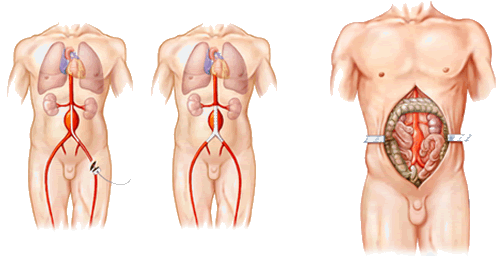
\includegraphics[height=150px]{comparacao_endoluminal_convencional.png}
\caption{Comparison between endoluminal and conventional surgery. Adapted from \citeonline{site2011}.}
\label{figura:comparacao_endoluminal_convencional}
\end{figure}

\section{Work purposes}
\label{section:work_purposes}
Make the work goals (main goal and specific goals) very clear.

\section{Work delimitations}
\label{section:work_limitations}
Every work has its limitations (although sometimes it might be hard for the author to notice).

\section{Justification}
Work relevance/contributions to the field.

\section{Overview of this work}
A good practice is to give a roadmap for this document. Write here a paragraph for each chapter, exposing its contents, main points and how it connects to other chapters (don't forget the appendix).